% Kernel-level API co-occurrence heatmap (lower-triangular matrix)
% APIs (col/row 0–12): CUDA, HIP, SYCL, OpenCL, OpenMP, OMP-Target,
%                      OpenACC, Kokkos, RAJA, TBB, Thrust, stdpar, Sequential
% NaN = upper triangle (rendered white); y dir=reverse puts CUDA at top-left
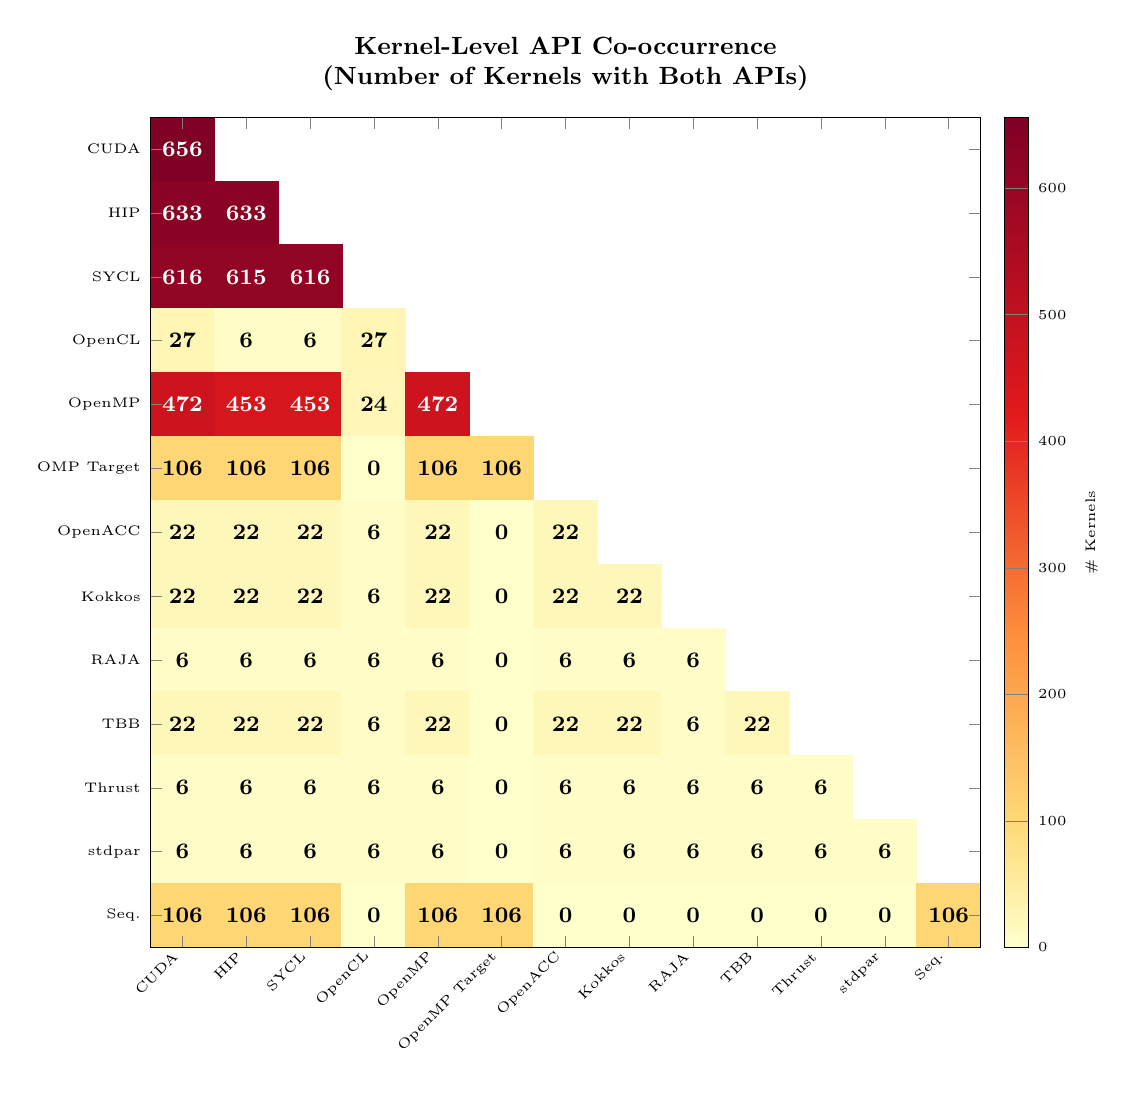
\begin{tikzpicture}
\begin{axis}[
  width=\columnwidth,
  height=\columnwidth,
  enlargelimits=false,
  axis on top,
  y dir=reverse,
  tick label style={font=\tiny},
  title style={font=\small\bfseries, align=center},
  colorbar,
  colorbar style={
    font=\tiny, width=0.3cm,
    ylabel={\# Kernels},
    ylabel style={font=\tiny},
  },
  xtick={0,1,2,3,4,5,6,7,8,9,10,11,12},
  xticklabels={CUDA,HIP,SYCL,OpenCL,OpenMP,{OpenMP Target},OpenACC,Kokkos,RAJA,TBB,Thrust,stdpar,Seq.},
  xticklabel style={font=\tiny, rotate=45, anchor=east},
  ytick={0,1,2,3,4,5,6,7,8,9,10,11,12},
  yticklabels={CUDA,HIP,SYCL,OpenCL,OpenMP,{OMP Target},OpenACC,Kokkos,RAJA,TBB,Thrust,stdpar,Seq.},
  yticklabel style={font=\tiny},
  xmin=-0.5, xmax=12.5,
  ymin=-0.5, ymax=12.5,
  colormap={ylOrRd}{
    rgb255(0)=(255,255,204)
    rgb255(100)=(254,217,118)
    rgb255(250)=(253,141,60)
    rgb255(420)=(227,26,28)
    rgb255(656)=(128,0,38)
  },
  point meta min=0, point meta max=656,
  title={Kernel-Level API Co-occurrence\\(Number of Kernels with Both APIs)},
]
  %% Color matrix — NaN for upper triangle (above diagonal → rendered white)
  \addplot[matrix plot*, mesh/cols=13, point meta=explicit] coordinates {
    % y=0: CUDA diagonal only
    (0,0)[656]   (1,0)[nan]   (2,0)[nan]   (3,0)[nan]   (4,0)[nan]   (5,0)[nan]   (6,0)[nan]   (7,0)[nan]   (8,0)[nan]   (9,0)[nan]   (10,0)[nan]  (11,0)[nan]  (12,0)[nan]
    % y=1: HIP
    (0,1)[633]   (1,1)[633]   (2,1)[nan]   (3,1)[nan]   (4,1)[nan]   (5,1)[nan]   (6,1)[nan]   (7,1)[nan]   (8,1)[nan]   (9,1)[nan]   (10,1)[nan]  (11,1)[nan]  (12,1)[nan]
    % y=2: SYCL
    (0,2)[616]   (1,2)[615]   (2,2)[616]   (3,2)[nan]   (4,2)[nan]   (5,2)[nan]   (6,2)[nan]   (7,2)[nan]   (8,2)[nan]   (9,2)[nan]   (10,2)[nan]  (11,2)[nan]  (12,2)[nan]
    % y=3: OpenCL
    (0,3)[27]    (1,3)[6]     (2,3)[6]     (3,3)[27]    (4,3)[nan]   (5,3)[nan]   (6,3)[nan]   (7,3)[nan]   (8,3)[nan]   (9,3)[nan]   (10,3)[nan]  (11,3)[nan]  (12,3)[nan]
    % y=4: OpenMP
    (0,4)[472]   (1,4)[453]   (2,4)[453]   (3,4)[24]    (4,4)[472]   (5,4)[nan]   (6,4)[nan]   (7,4)[nan]   (8,4)[nan]   (9,4)[nan]   (10,4)[nan]  (11,4)[nan]  (12,4)[nan]
    % y=5: OMP Target
    (0,5)[106]   (1,5)[106]   (2,5)[106]   (3,5)[0]     (4,5)[106]   (5,5)[106]   (6,5)[nan]   (7,5)[nan]   (8,5)[nan]   (9,5)[nan]   (10,5)[nan]  (11,5)[nan]  (12,5)[nan]
    % y=6: OpenACC
    (0,6)[22]    (1,6)[22]    (2,6)[22]    (3,6)[6]     (4,6)[22]    (5,6)[0]     (6,6)[22]    (7,6)[nan]   (8,6)[nan]   (9,6)[nan]   (10,6)[nan]  (11,6)[nan]  (12,6)[nan]
    % y=7: Kokkos
    (0,7)[22]    (1,7)[22]    (2,7)[22]    (3,7)[6]     (4,7)[22]    (5,7)[0]     (6,7)[22]    (7,7)[22]    (8,7)[nan]   (9,7)[nan]   (10,7)[nan]  (11,7)[nan]  (12,7)[nan]
    % y=8: RAJA
    (0,8)[6]     (1,8)[6]     (2,8)[6]     (3,8)[6]     (4,8)[6]     (5,8)[0]     (6,8)[6]     (7,8)[6]     (8,8)[6]     (9,8)[nan]   (10,8)[nan]  (11,8)[nan]  (12,8)[nan]
    % y=9: TBB
    (0,9)[22]    (1,9)[22]    (2,9)[22]    (3,9)[6]     (4,9)[22]    (5,9)[0]     (6,9)[22]    (7,9)[22]    (8,9)[6]     (9,9)[22]    (10,9)[nan]  (11,9)[nan]  (12,9)[nan]
    % y=10: Thrust
    (0,10)[6]    (1,10)[6]    (2,10)[6]    (3,10)[6]    (4,10)[6]    (5,10)[0]    (6,10)[6]    (7,10)[6]    (8,10)[6]    (9,10)[6]    (10,10)[6]   (11,10)[nan] (12,10)[nan]
    % y=11: stdpar
    (0,11)[6]    (1,11)[6]    (2,11)[6]    (3,11)[6]    (4,11)[6]    (5,11)[0]    (6,11)[6]    (7,11)[6]    (8,11)[6]    (9,11)[6]    (10,11)[6]   (11,11)[6]   (12,11)[nan]
    % y=12: Sequential
    (0,12)[106]  (1,12)[106]  (2,12)[106]  (3,12)[0]    (4,12)[106]  (5,12)[106]  (6,12)[0]    (7,12)[0]    (8,12)[0]    (9,12)[0]    (10,12)[0]   (11,12)[0]   (12,12)[106]
  };
  %% White labels for dark cells (value >= 200)
  \addplot[
    only marks, mark=none, point meta=explicit,
    nodes near coords={\pgfmathfloattoint{\pgfplotspointmeta}\pgfmathresult},
    nodes near coords align={center},
    every node near coord/.style={font=\footnotesize\bfseries, text=white, inner sep=0pt}
  ] coordinates {
    (0,0)[656]  (0,1)[633]  (1,1)[633]  (0,2)[616]  (1,2)[615]  (2,2)[616]
    (0,4)[472]  (1,4)[453]  (2,4)[453]  (4,4)[472]
  };
  %% Black labels for light cells (value < 200) — lower triangle only
  \addplot[
    only marks, mark=none, point meta=explicit,
    nodes near coords={\pgfmathfloattoint{\pgfplotspointmeta}\pgfmathresult},
    nodes near coords align={center},
    every node near coord/.style={font=\footnotesize\bfseries, text=black, inner sep=0pt}
  ] coordinates {
    % Row 3 (OpenCL)
    (0,3)[27]    (1,3)[6]     (2,3)[6]     (3,3)[27]
    % Row 4 light cell
    (3,4)[24]
    % Row 5 (OMP Target)
    (0,5)[106]   (1,5)[106]   (2,5)[106]   (3,5)[0]     (4,5)[106]   (5,5)[106]
    % Row 6 (OpenACC)
    (0,6)[22]    (1,6)[22]    (2,6)[22]    (3,6)[6]     (4,6)[22]    (5,6)[0]     (6,6)[22]
    % Row 7 (Kokkos)
    (0,7)[22]    (1,7)[22]    (2,7)[22]    (3,7)[6]     (4,7)[22]    (5,7)[0]     (6,7)[22]    (7,7)[22]
    % Row 8 (RAJA)
    (0,8)[6]     (1,8)[6]     (2,8)[6]     (3,8)[6]     (4,8)[6]     (5,8)[0]     (6,8)[6]     (7,8)[6]     (8,8)[6]
    % Row 9 (TBB)
    (0,9)[22]    (1,9)[22]    (2,9)[22]    (3,9)[6]     (4,9)[22]    (5,9)[0]     (6,9)[22]    (7,9)[22]    (8,9)[6]     (9,9)[22]
    % Row 10 (Thrust)
    (0,10)[6]    (1,10)[6]    (2,10)[6]    (3,10)[6]    (4,10)[6]    (5,10)[0]    (6,10)[6]    (7,10)[6]    (8,10)[6]    (9,10)[6]    (10,10)[6]
    % Row 11 (stdpar)
    (0,11)[6]    (1,11)[6]    (2,11)[6]    (3,11)[6]    (4,11)[6]    (5,11)[0]    (6,11)[6]    (7,11)[6]    (8,11)[6]    (9,11)[6]    (10,11)[6]   (11,11)[6]
    % Row 12 (Sequential)
    (0,12)[106]  (1,12)[106]  (2,12)[106]  (3,12)[0]    (4,12)[106]  (5,12)[106]  (6,12)[0]    (7,12)[0]    (8,12)[0]    (9,12)[0]    (10,12)[0]   (11,12)[0]   (12,12)[106]
  };
\end{axis}
\end{tikzpicture}
